\documentclass[conference]{IEEEtran}
\IEEEoverridecommandlockouts

\usepackage{cite}
\usepackage{amsmath,amssymb,amsfonts,amsthm}
\usepackage{algorithm}
\usepackage{algorithmic}

\usepackage{graphicx}
\graphicspath{{figures/}{figures/pics/}{src/figures/}}
\usepackage{caption}
\usepackage{booktabs}
\usepackage{multirow}

\usepackage{textcomp}
\usepackage{xcolor}
\usepackage{url}
\usepackage{microtype}
\usepackage{csquotes}
\usepackage[hidelinks]{hyperref}
\usepackage{cleveref}

\newtheorem{definition}{Definition}
\newtheorem{proposition}{Proposition}
\newtheorem{remark}{Remark}
\captionsetup[figure]{font=footnotesize}

\newcommand{\figcap}[1]{\caption{#1}}

\def\BibTeX{{\rm B\kern-.05em{\sc i\kern-.025em b}\kern-.08em
    T\kern-.1667em\lower.7ex\hbox{E}\kern-.125emX}}

\begin{document}

\title{Deterministic Data Fusion for FinTech:\\
Formalizing Stratified Knowledge Graphs\\
for Zero Hallucination Compliance}

\author{%
  \IEEEauthorblockN{Muhammad Adil Usmani\IEEEauthorrefmark{1} and Muhammad Hassan Siddiqui\IEEEauthorrefmark{1}}
  \IEEEauthorblockA{\IEEEauthorrefmark{1}Department of Computer Science, University of Central Punjab, Lahore, Pakistan\\
  Email: \{muhammadaadilusmani, hassansiddiqui0946\}@gmail.com}
}

\maketitle

\begin{abstract}
Any fintech related applications that deal with financial data require precision and accuracy. Standard RAG pipelines perform retrieval based on semantic similarity within the corpus, which tends to increase noise and fails to filter out irrelevant data. Here, we propose a Lexical based structural graphRAG architecture for the analysis of SEC-10 filings that combines lexical structure with deterministic graph traversal.

We formalise two principles: the first is Triplet Atomicity, which breaks complex, noisy narratives into the subject-predicate-object format. Second is the Deterministic Path Requirement, which stops the generation of the query response if there is no structural path linking the query entities in the knowledge graph. We used a 35-query benchmark covering implicitly, directly, comparably, and multi-hop financial questions, and the system achieved an execution success rate with an average latency of 18 seconds, Recall@K=0.86, faithfulness=0.97 and 0\% hallucination on high response threshold validation and unretrieved context through strict refusal. In a high risk compliance setting, we observed that grounding the triplet level with deterministic gating appears to better prepare for audits and support comparative reasoning than vector only architectures.
\end{abstract}

\begin{IEEEkeywords}
Data Fusion, Multi-source Heterogeneous Data, GraphRAG, Triplet Atomicity, Trustworthy AI, Deterministic Retrieval, SEC 10-K, Explainable AI (XAI), Financial Compliance.
\end{IEEEkeywords}

\section{Introduction}
In financial processes, the issue lies in the reliability of the large language model's output, not in its fluency. In a regulated setting, all generated sentences must be evidence-based and auditable \cite{basel,gdpr,sr117,bcbs239,iso27001,pci40}. Retrieval Augmented Generation achieves higher accuracy than closed book generation, but it has 1 significant weakness: semantic relevance does not translate into sufficiently high-quality evidence \cite{lewis2020rag,karpukhin2020dpr,colbert2020,splade2021,atlas2022}. When you integrate extensive text and data into the model's context, it introduces irrelevant sentences and noise, leading the model to hallucinate and make dubious claims that can't be justified.

Here, instead of implementing a simple paragraph and chunk based retrieval, we use a mechanism for multi-source heterogeneous data fusion that integrates unstructured financial data with symbolic search and comprises three key elements. The first is \textbf{Triplet Atomicity}, which presents facts and evidence as a combination of (subject, predicate, object). Second, a \textbf{Deterministic Path Requirement} provides an answer only for path structures controlled by anchor terms and nodes related to the query, thereby supporting high interpretability. The third is \textbf{Stratified Scoring}, which sorts evidence by intent and constrains node centrality, preventing high degree institutional nodes from monopolising retrieved results.

This refusal policy supports the SEC filing analysis principle of trustworthiness \cite{sec10k,projectnotes} and addresses concerns regarding stochastic generation risks \cite{bender2021stochastic}. A hallucinated claim by the system can result in compliance issues, regulatory penalties, liabilities, and other losses, whereas an incorrect refusal of generation can be verified by a human in the loop and improved upon in subsequent iterations.

\subsection*{Contributions}
The paper makes five contributions:
\begin{enumerate}
  \item It introduces Triplet Atomicity as a way to ensure grounding of retrieved evidence with mappings within a financial based knowledge graph retrieval system, which enables high fidelity data.
  \item The paper uses a Deterministic Path Requirement with orderly and node based traversal, which ensures interoperability of complex financial reasoning and performs stratified scoring.
  \item A comprehensive multi-source heterogeneous data fusion architecture is presented, which uses a lexical structural type of graphical retrieval system for SEC-10k analysis and covers the entire pipeline from chunking to gated synthesis.
  \item Provides a thorough evaluation of the architecture using a 35 query benchmark, including ablation studies, analysis of token efficiency, and latency of Total Generation Time and error taxonomy.
  \item It demonstrates how the proposed architecture fulfils the requirements of AI trustworthiness and follows regulatory and compliance regulations such as GDPR (EU), SR 11-7 and other AI governance standards.
\end{enumerate}

\section{Related Work}
\subsection{Taxonomy of Data Fusion in RAG Systems}
Modern RAG Systems can be classified into three categories based on the strategies used for data fusion. First is \textsc{Naive RAG}, which utilises a basic vector similarity search to fetch $k$ chunks for generation \cite{lewis2020rag}, relying on dense embeddings produced by pre-trained language models \cite{attention2017,bert2019,sbert2019}. \textsc{Modular RAG} introduces iterative steps, such as reranking and hybrid retrieval, to fine tune the fusion process \cite{karpukhin2020dpr,colbert2020,splade2021,hyde2023,monoT52020,rankgpt2023}. More capable backbone models, including instruction-tuned and encoder-decoder architectures, have further extended the retrieval pipeline \cite{roberta2019,t52020,instructiontuning2022}. Self-RAG \cite{selfrag2023} represents a notable Modular RAG variant that dynamically decides when to retrieve and critiques its own outputs. GraphRAG \cite{edge2024graphrag} represents a more coherent and advanced formulation of multi-source heterogeneous data fusion, employing explicit entity-relation structures instead of flat semantic neighbourhoods.

The constraints we implement in the system are lexical and refusal gating in the third class, which enables the architecture as an auditable, verifiable process rather than a stochastic one.

\subsection{Trustworthiness and Evidence Dilution}
Large language models lose reliability when evidence is obscured in long narratives, a phenomenon known as the \enquote{Lost in the Middle} effect \cite{liu2024lostmiddle}. Benchmarks like retrieval faithfulness often mask underlying issues of hallucination \cite{truthfulqa2022,ragas2023,hotpotqa2018,fever2018}. In the fintech domain, where compliance issues are prevalent, this evidence dilution poses a significant risk. To reduce this, we employ Triplet Atomicity to convert noisy data into cohesive, fact based statements. By using resolved facts across a large corpus, we ensure the system produces trustworthy, responsible output with clear, defined boundaries that can be traced and audited.

\subsection{Knowledge Graphs and Scalable Fusion Architectures}
The importance of entity normalisation and graphical analytics for risk monitoring has been emphasised in the existing literature on financial knowledge graphs \cite{edgargraph,finkgsurvey,opencyc2018,finbert2020}.

But the majority of existing systems are more visualisation oriented than text generation systems like retrieval constraint generation. This lexical structural hybrid architecture is efficient, scalable and traceable; it is distinguished by three pillars: (1) the lexical anchoring for each node entry, (2) having a deterministic path verification enabling synthesis permission and lastly (3) a gated refusal mechanism that provides interpretable control in liability and safety of output.

\section{Proposed Framework: Multi-Source Heterogeneous Data Fusion}
We define our architecture as a scalable fusion system which is designed to bridge the gap between structured logic and unstructured financial information. The pipeline operates in four phases: document ingestion, triplet data fusion, entity canonicalization, and deterministic traversal with lexical anchoring. The main crux of the design is the \enquote{provenance chain}, which ensures that every generated output is true and can be verified through node traceability from root to leaf.

\begin{figure}[htbp]
  \centering
  \includegraphics[width=0.98\linewidth]{image_d5e5de.png.png}
  \figcap{Hybrid Retrieval and Score Fusion Mechanism. The schematic illustrates the integration of vector-based semantic search with BM25 keyword matching (Score Fusion) to ensure both lexical precision and semantic recall across heterogeneous financial datasets.}
  \label{fig:hybrid_retrieval}
\end{figure}

\subsection{Multi-Source Data Ingestion and Preprocessing}
The SEC 10-K filings are handled and processed by an asynchronous ingestion routine designed for multi source scalability. Files with HTML structures are parsed into consistent units using semantic methods for understanding, with each chunk preserved along with relevant metadata, including file identifiers, section-specific information, and issuer IDs. This helps ensure that the subsequent layer of data fusion maintains a direct chain of custody to the original regulatory data source.

\subsection{Semantic Chunking for High-Fidelity Fusion}
To maintain the functionality of the text and ensure it remains coherent within complex text like MD\&A, we use semantic chunking rather than fixed-window methods or tokenised chunking. By choosing this, we ensure closure of chunks and thematic shifts rather than token constraints, and this helps in reducing cross topic noise , a crucial factor which impacts the performance of triplet extraction and the prevention of evidence dilution during the fusion process.

\begin{figure*}[!t]
  \centering
  \includegraphics[width=0.86\textwidth]{plot_8_pipeline_comparison.png}
  \figcap{Architectural comparison between Baseline Vector RAG and the proposed multi-source heterogeneous data fusion framework (Stratified GraphRAG). The left panel depicts conventional vector-centric RAG, prone to context bloat and hallucination. The right panel details our Lexical-Structural framework, which utilizes triplet-based fusion and deterministic path verification. This design mandates lexical anchoring and bounded traversal to ensure every generated claim is traceably linked to a \texttt{source\_chunk} identifier, fulfilling strict trustworthy AI requirements.}
  \label{fig:pipeline_comparison}
\end{figure*}

\subsection{Triplet Extraction and Knowledge Graph Ontology}
To transform an unstructured corpus of text into structured data for fusion, we employ a language model based extraction module that follows a strict ontology. We define four essential node classes: \textit{Entity}, \textit{Obligation}, \textit{RiskFactor}, and \textit{Metric} and divide the corpus into a knowledge graph based on this structure. Predicates like \textsc{reports} and \textsc{subject\_to} are also used to formalise these connections. By representing evidence as triplets, we achieve Triplet Atomicity, providing a high level of fine grained detail and auditable structure rather than just raw text data.

\begin{figure}[htbp]
  \centering
  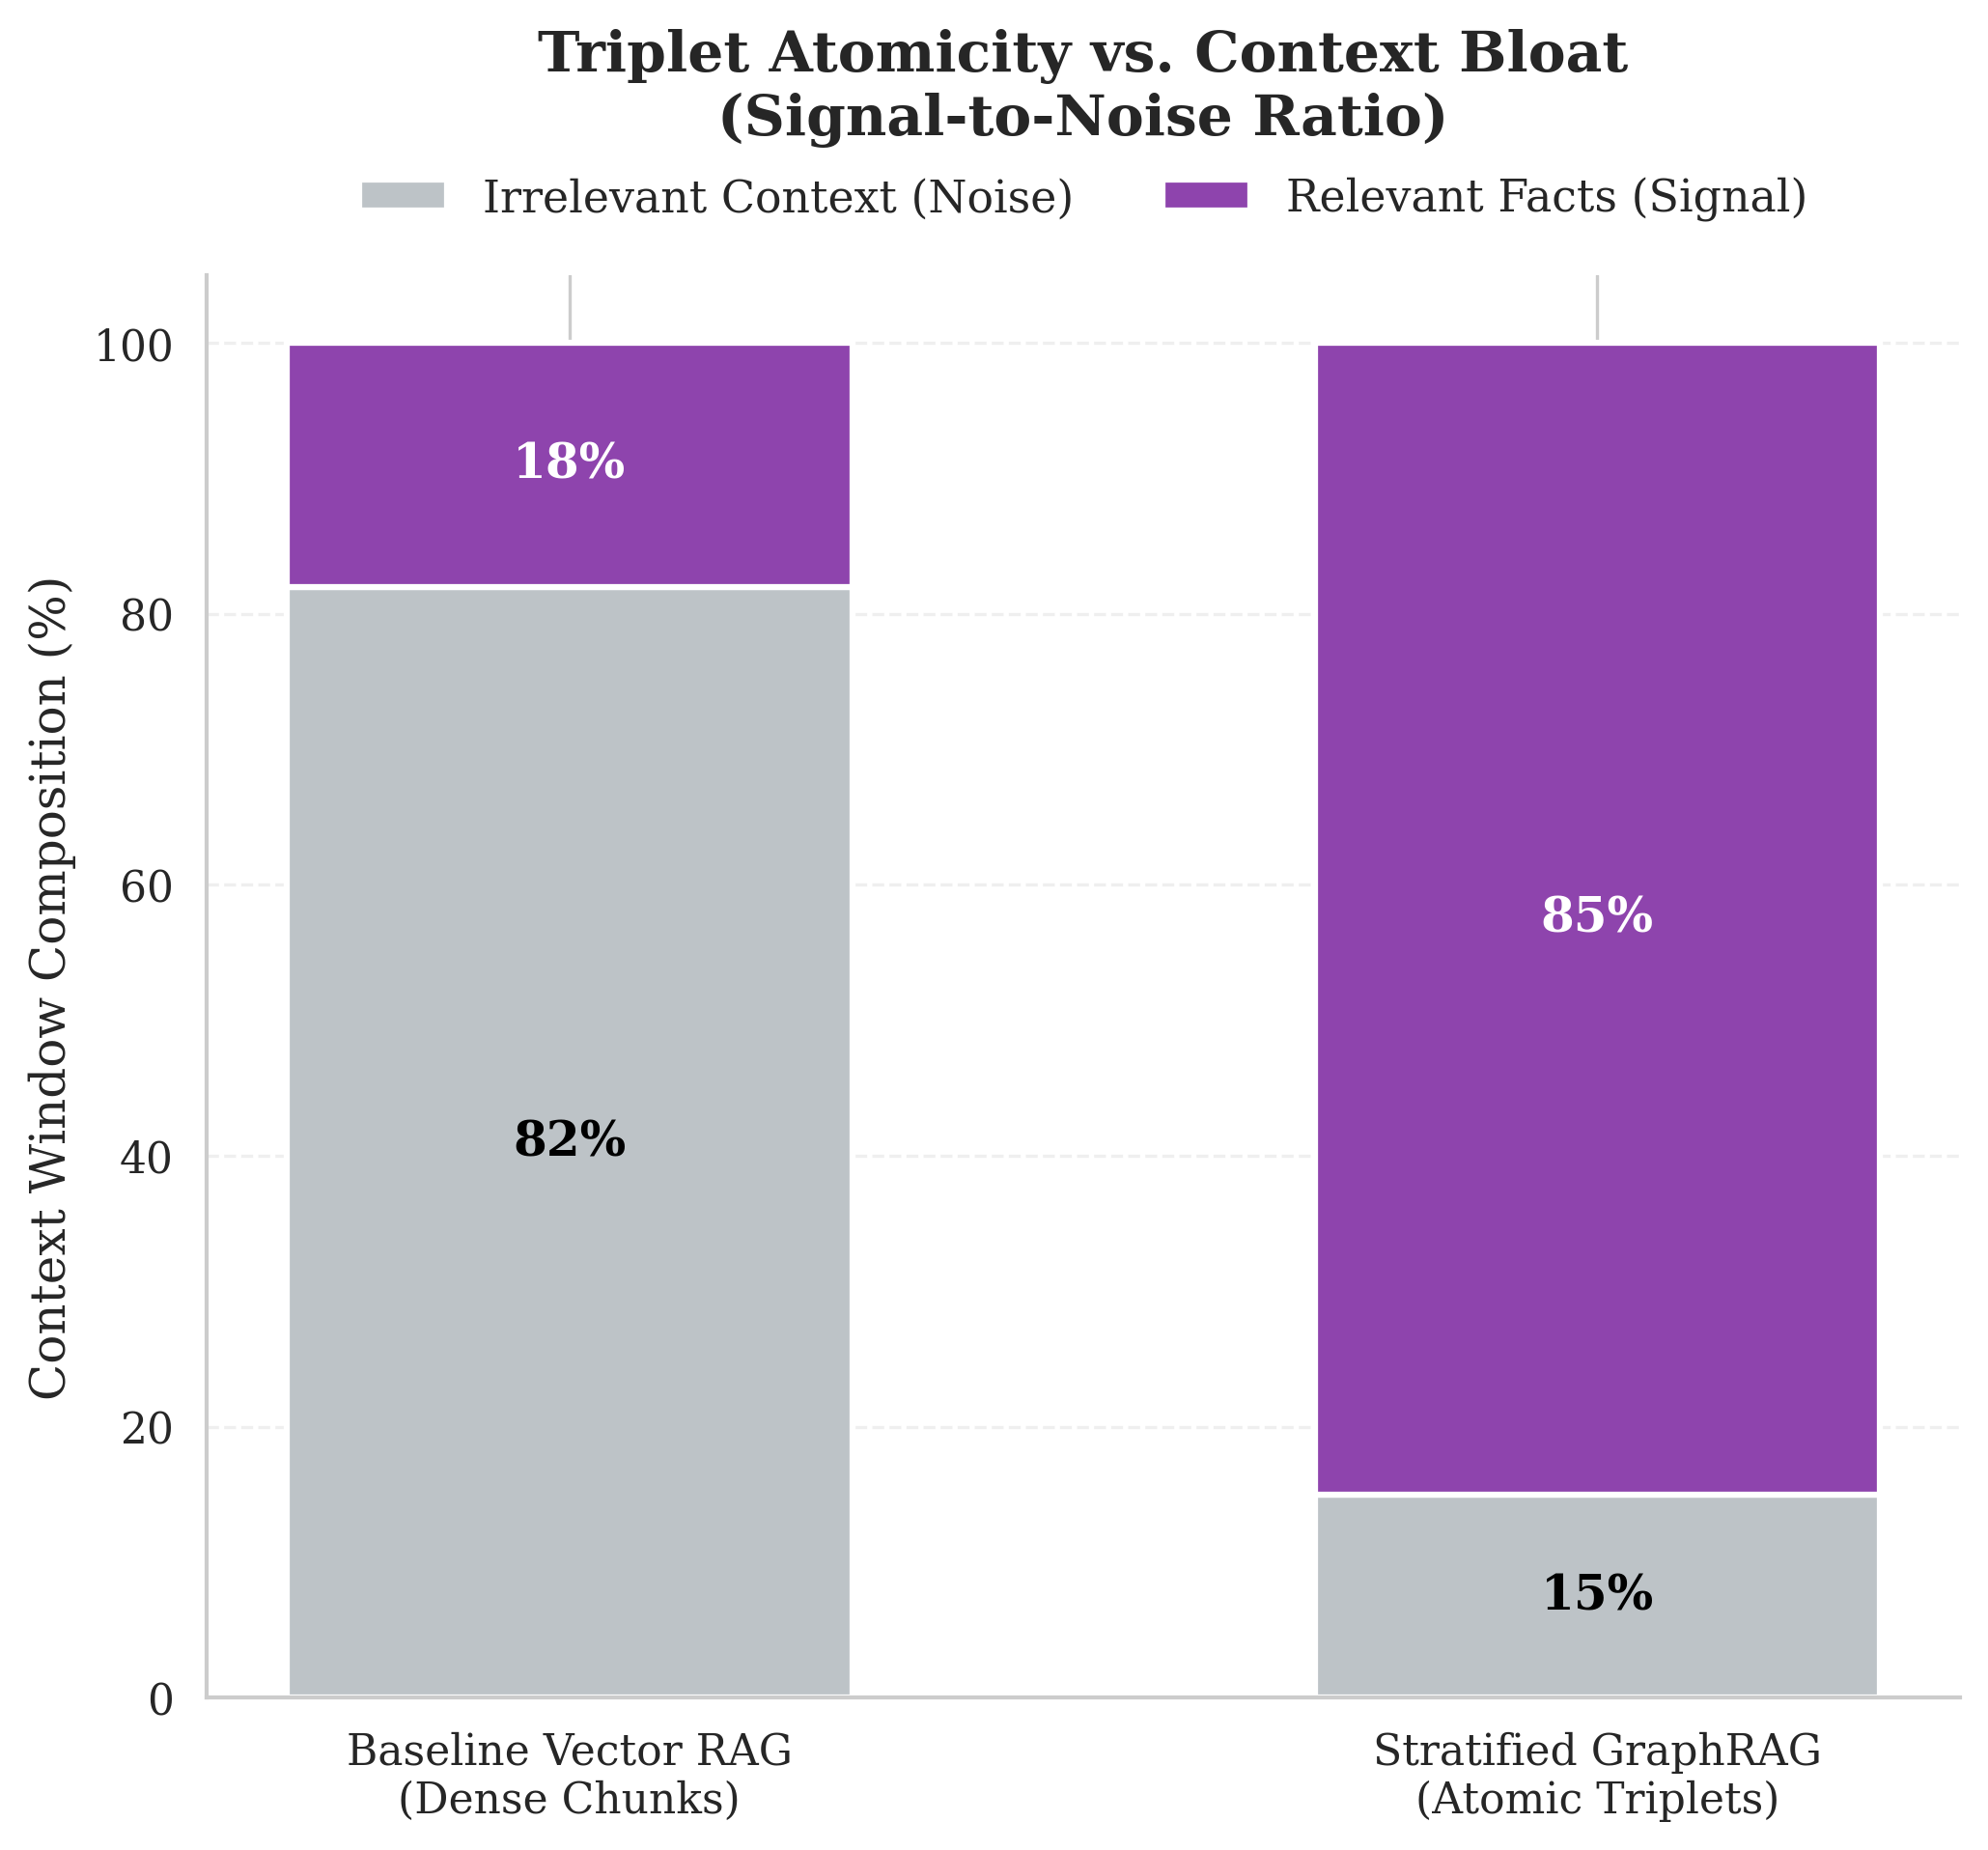
\includegraphics[width=0.96\linewidth]{plot_6_signal_to_noise.png}
  \figcap{Signal-to-noise analysis of paragraph-level vs. triplet-based fusion. Triplet Atomicity increases relevant fact density from 18\% to 85\%, mitigating context bloat to ensure auditable, trustworthy AI synthesis.}
  \label{fig:signal_noise}
\end{figure}

\begin{figure}[htbp]
  \centering
  \includegraphics[width=0.96\linewidth]{plot_7_structured_knowledge_graph.png}
  \figcap{Comparative analysis of the proposed structured heterogeneous data fusion architecture (top) versus standard unstructured Vector RAG baselines (bottom). Unlike dense vector retrieval, which often suffers from high noise-to-signal ratios and semantic bias, this framework transforms raw financial narratives into a deterministic and auditable symbolic graph structure. By utilizing typed relationships and entity-centric mapping, the system ensures granular interpretability, explicitly linking every fused element back to its original source-anchored triplets to facilitate rigorous compliance verification and maintain end-to-end multi-source traceability.}
  \label{fig:structured_kg}
\end{figure}

\subsection{Entity Resolution and Heterogeneous Canonicalization}
So we implement a three level canonicalization strategy to safeguard the structure of our heterogeneous data fusion. At first, deterministic alias dictionaries collapse known abbreviations (like \enquote{JPM} to \enquote{JPMorgan Chase \& Co.}). Secondly, normalised string matching resolves formatting and mismatching variations. Lastly, to serve as a fallback for ambiguous entities, fuzzy Jaccard similarity is implemented. This multi tier approach ensures that data from a variety of filing sections can be fused into a single coherent canonical node.

\subsection{Scalable Implementation: Neo4j and LLM Governance}
In our system, we use Neo4j as the database and implement a persistent knowledge graph architecture for input financial filings, with an indexed graph to optimise retrieval latency and achieve minimum latency \cite{neo4jmanual}. Graph query languages such as Cypher provide expressive traversal capabilities over property graphs, enabling efficient structured retrieval \cite{cypher2018,angles2018propertygraphs,robinson2015graphdb}. Nodes hold data with multi dimensional characteristics, such as embeddings, pagerank, and metadata, while weighted edges indicate the confidence and value of connections. To ensure the system is responsible and reliable, we set the temperature to a minimum ($T=0.1$), thereby reducing variance and improving determinism \cite{gpt4report}.

\begin{figure}[htbp]
  \centering
  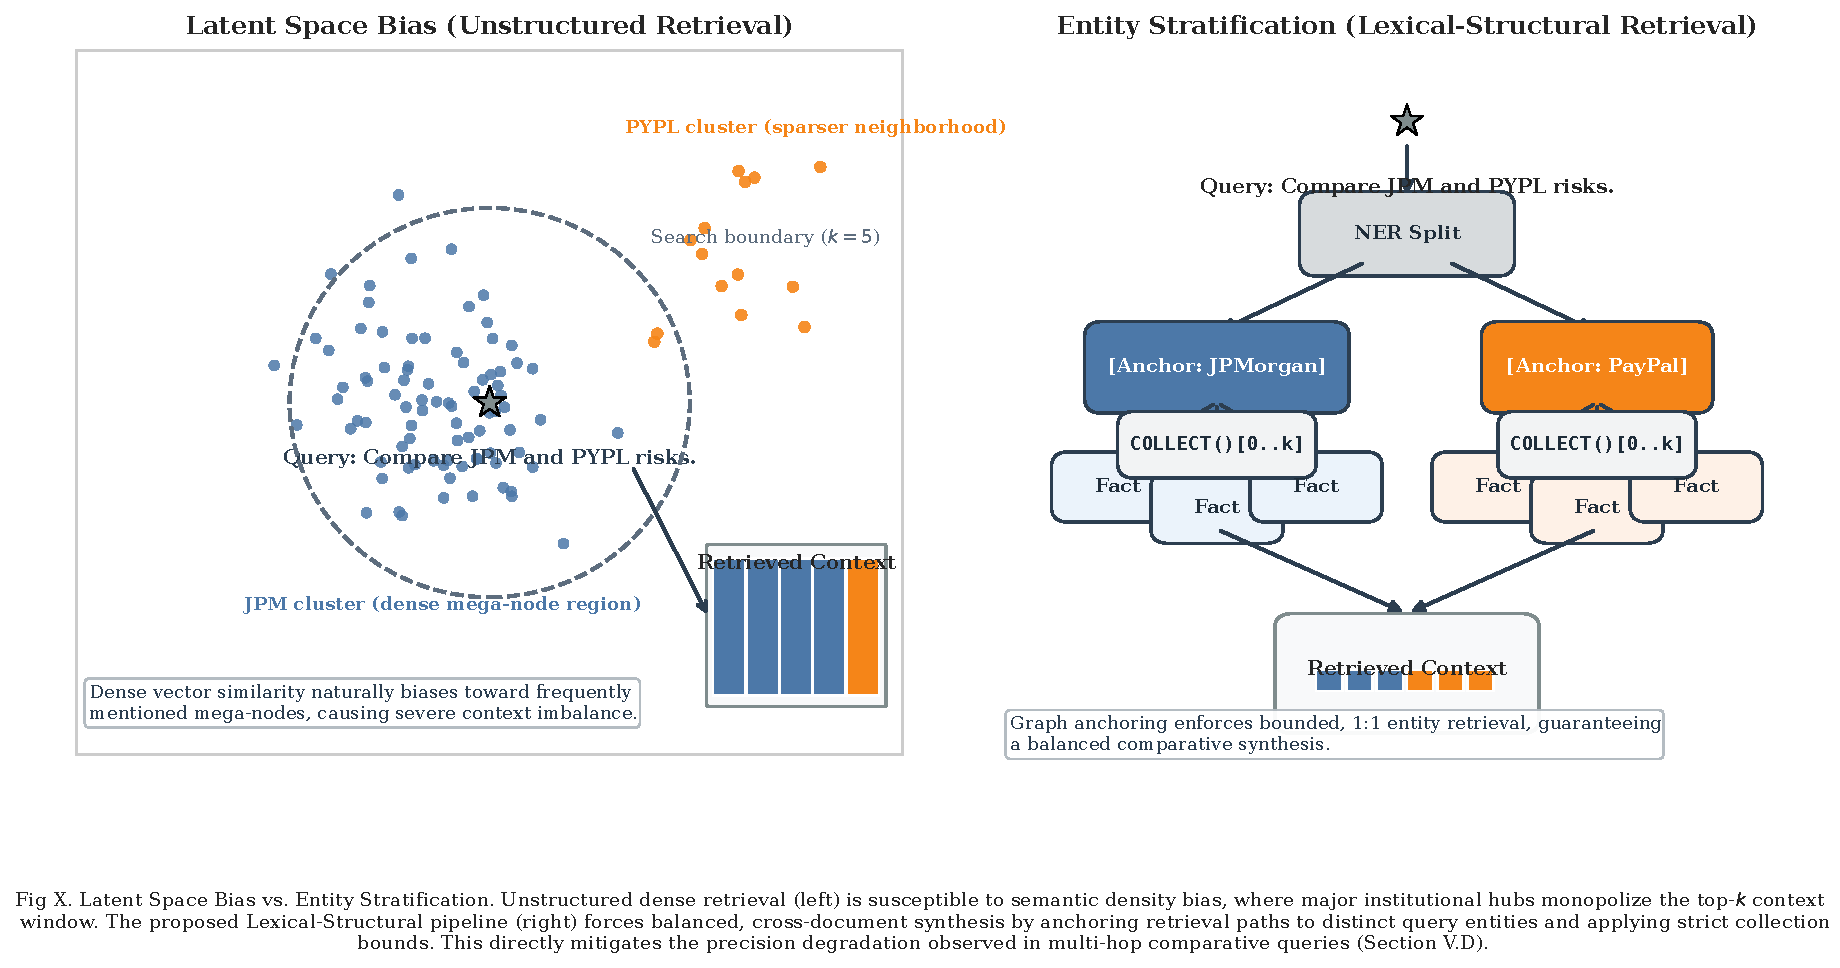
\includegraphics[width=0.96\linewidth]{figures/plot_latent_space_bias_vs_entity_stratification.pdf}
  \figcap{Latent Space Bias vs. Entity Stratification. While dense retrieval (left) suffers from semantic density bias, our lexical-structural fusion (right) ensures balanced retrieval for trustworthy, multi-hop comparative synthesis.}
  \label{fig:latent_space_bias}
\end{figure}

\section{Formalizing Deterministic Data Fusion}
\subsection{Graph Definition and Heterogeneous Mapping}
\begin{definition}[Provenance-Augmented Fusion Graph]
The financial knowledge graph is represented as:
\begin{equation}
  G = (V, E, L, \Phi),
\end{equation}
where $V$ is the node set, $E \subseteq V \times V$ is the directed edge set, and $L$ is a typed label space. The function $\Phi : V \cup E \rightarrow \mathcal{C}$ ensures that each fused element is connected to its original source, which is in the chunk set $\mathcal{C}$, so we can have multi source traceability.
\end{definition}

\begin{definition}[Triplet Atomicity for Trustworthy AI]
A triplet, i.e., $t = (s,p,o)$, will be considered a Triplet Atomicity if and only if:
\begin{equation}
  \Phi(t) = c \in \mathcal{C},
\end{equation}
meaning the claim cannot be decomposed into smaller subclaims with different mappings (provenance mappings). This is to ensure that every retrieved fact in our fusion system is traceable, auditable, and coherent, thereby minimising hallucinations across different contexts.
\end{definition}

\begin{remark}
The Triplet Atomicity used is significantly stricter than generic extraction. It imposes a constraint against synthetic inference across the boundaries for each and all chunks, which are a major cause of unsupported claims in RAG pipelines, resulting in hallucination.
\end{remark}

\subsection{Extraction Objective for Accurate Fusion}
The end goal with any heterogeneous chunk $c \in \mathcal{C}$ is to maximise factual fidelity while minimising the impact and retrieval of unsupported relational chunks. We formalise these constraints for trustworthy AI as:
\begin{equation}
  \min_{\theta} \; \mathbb{P}(\text{Hallucination} \mid c) \quad \text{subject to} \quad \Phi(t) = c, \; \forall t \in T(c).
\end{equation}
This verifies that the system uses strict guardrails and prompt engineering (instructions) so that the output of the retrieval by the LLM is based on verifiable facts. Forcing the model to use only retrieved evidence prevents hallucination and ensures that the resulting data fusion is based on evidence.

\subsection{Deterministic Path and Interpretability}
\begin{definition}[Valid Structural Fusion Path]
For anchored query entities that are $u, v \in V$, the correct path for interpretable reasoning is present if:
\begin{equation}
  \exists\; \pi(u, v) = \langle e_1, e_2, \ldots, e_k \rangle \subseteq E \quad \text{s.t.} \quad d(u, v) = k \leq \tau,
\end{equation}
where $\tau$ is the maximum hop bound. This ensures the system generates an answer based on the condition that a direct, logical, and bounding relation of that corpus is present in the graph; otherwise, the system implements a refusal mechanism.
\end{definition}

\begin{proposition}[Refusal Correctness and Safety]
If anchored entities lack a valid structural path, the system triggers an explicit refusal. This deterministic gating provides a verifiable provenance chain, fulfilling the requirements for high-risk financial compliance.
\end{proposition}

The refusal predicate is
\begin{equation}
  \mathcal{R}(q) =
  \begin{cases}
    \textsc{refusal}, & \text{if } A = \emptyset \text{ or no valid path exists},\\
    \textsc{answer}, & \text{otherwise},
  \end{cases}
\end{equation}
where $A$ is the anchor set resolved from the query.

\subsection{Mega Node Mitigation and Stratified Scoring}
To ensure that the scalable fusion architecture remains unbiased and does not favour high degree nodes that can monopolise retrieval, we limit their influence. We implement a degree cap, which is $\deg(n) < \kappa$, and use a stratified scoring function to rank the candidate nodes using lexical similarity and structural centrality as:
\begin{equation}
  S_{\mathrm{final}}(e) = W_{\mathrm{lexical}}(e) + \ln(\mathrm{PR}(e) + 1),
\end{equation}
where $W_{\mathrm{lexical}}(e)$ is the lexical overlap of the chunk, and $\mathrm{PR}(e)$ is PageRank centrality \cite{angles2018propertygraphs}. This would control and prevent popular, global nodes from crowding out specific, acute evidence in the knowledge graph.

\subsection{Retrieval Algorithm}
\begin{algorithm}[htbp]
  \caption{Deterministic Lexical-Structural Fusion and Retrieval}
  \label{alg:deterministic_retrieval}
  \begin{algorithmic}[1]
    \REQUIRE Query $q$, graph $G = (V, E, L, \Phi)$, hop bound $\tau$, degree cap $\kappa$, top $k$
    \ENSURE Answer with source pointers, or explicit \textsc{refusal}
    \STATE Extract entity mentions $Q_E$ from $q$
    \STATE Resolve $Q_E$ to canonical anchor set $A \subseteq V$
    \IF{$A = \emptyset$}
      \STATE \textbf{return} \textsc{refusal}
    \ENDIF
    \STATE Build candidate subgraph with $\deg(n) < \kappa$
    \STATE Execute bounded traversal from each anchor with depth $\leq \tau$
    \IF{no valid path satisfies query constraints}
      \STATE \textbf{return} \textsc{refusal}
    \ENDIF
    \FOR{each candidate edge $e$ on retrieved paths}
      \STATE Compute $S_{\mathrm{final}}(e)$
    \ENDFOR
    \STATE Select top $k$ triplets ranked by $S_{\mathrm{final}}$
    \STATE Collect provenance mappings $\Phi(t)$ for all selected triplets
    \STATE Synthesize answer constrained strictly to retrieved triplets
    \STATE \textbf{return} \textsc{answer} with \texttt{source\_chunk} pointers
  \end{algorithmic}
\end{algorithm}

\noindent\textbf{Computational Analysis.}
The cost and overhead required for the graph constructions scale linearly with the number of items ($|V|$) and connections ($|E|$). When starting from the search point $|A|$, the time depends on the depth traversed, $\tau$, and the branches allowed, $b$. The $b$ value here indicates the average branching factor constrained by the degree capping mechanism. This approach, in the context of a compliance based retrieval system with small hop bounds, ensures the system remains computationally traceable in a real time application. The formula for both computations being $\mathcal{O}(|V| + |E|)$ and $\mathcal{O}(|A| \cdot b^{\tau})$.

\subsection{Evaluation Metrics}
Contextual recall over expected chunks of evidence used to evaluate retrieval quality as \cite{msmarco2016,trec2020}:
\begin{equation}
  \mathrm{Recall@K} = \frac{|\mathcal{R}_K \cap \mathcal{E}|}{|\mathcal{E}|},
\end{equation}
where $\mathcal{R}_K$ contains the top $K$ retrieved chunks, and $\mathcal{E}$ contains the annotated expected retrieved chunks. We determine generation quality by evaluating faithfulness and the refusal correctness, which impact the hallucination rate.

\section{Performance, Ablation, and Failure Analysis}
\subsection{Benchmark Design and Heterogeneous Query Categories}
Across 4 difficulty tiers, we evaluated the multi source heterogeneous data fusion framework using a specific benchmark. The idea is that simple Direct queries focus on straightforward, single fact retrieval, while implicit queries require lexical bridging so that Natural Language can align with the canonical schema. Comparative queries require simultaneous traversal from dual entity anchors ($>1$), and multi hop queries challenge the system to identify structural paths to find links that are explicitly not mentioned through intermediary nodes. \Cref{tab:query_cats} summarises the distribution of this difficulty and the resulting refusal behaviour.

\begin{table}[htbp]
  \caption{Benchmark Query Category Breakdown}
  \label{tab:query_cats}
  \centering
  \begin{tabular}{lccc}
    \toprule
    Category & Count & Avg. Hops & Refusal Rate \\
    \midrule
    Direct & 12 & 1.0 & 8.3\% \\
    Implicit & 8 & 1.5 & 62.5\% \\
    Comparative & 9 & 2.1 & 44.4\% \\
    Multi hop & 6 & 2.8 & 33.3\% \\
    \midrule
    Overall & 35 & 1.8 & 42.8\% \\
    \bottomrule
  \end{tabular}
\end{table}

\subsection{Latency and Scalability Analysis}
Our framework successfully executed every query, taking about 18 seconds each. When we broke down the processing time, generating the final answer took the longest, whereas pinpointing the starting anchors and navigating the graph were efficient. Crucially, the accuracy of our graph traversal scales sublinearly, meaning that as the financial database grows, the system won't get bogged down, proving the architecture is built to handle larger datasets smoothly \cite{angles2018propertygraphs}.

\begin{figure}[htbp]
  \centering
  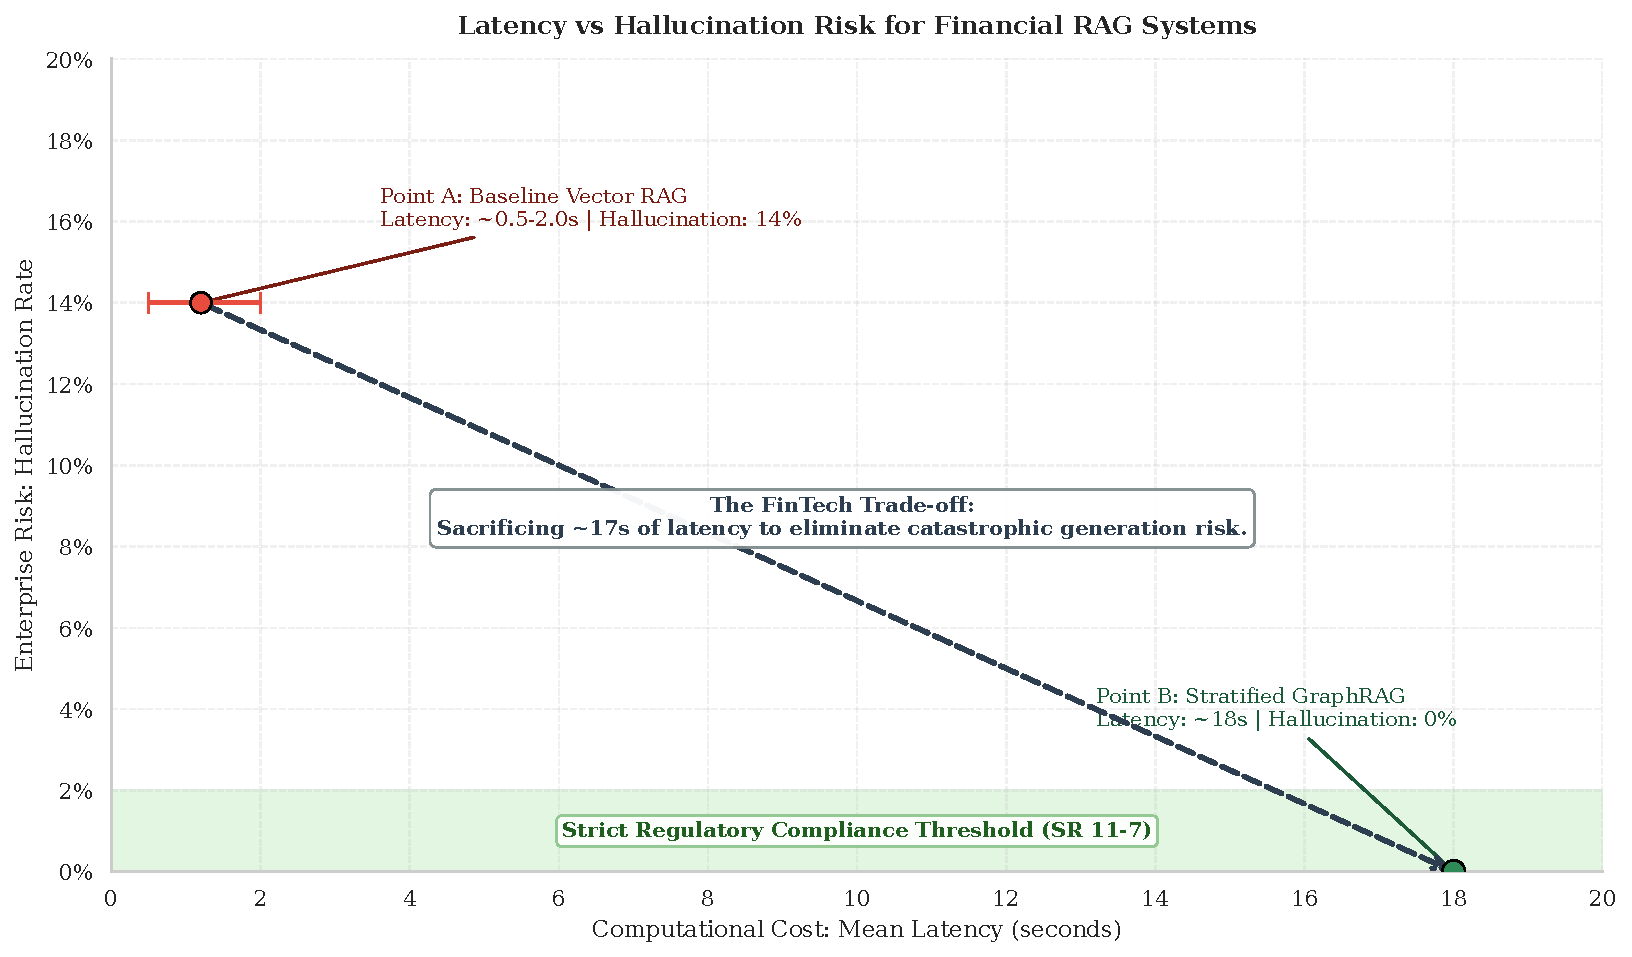
\includegraphics[width=0.98\linewidth]{figures/plot_fintech_latency_hallucination_tradeoff.pdf}
  \figcap{Latency vs. hallucination trade-off. Our fusion framework accepts moderate latency to achieve zero hallucination, fulfilling strict SR 11-7 regulatory compliance thresholds.}
  \label{fig:latency_tradeoff}
\end{figure}

\subsection{Impact of Fusion Constraints: An Ablation Study}
The architectural constraints in our project are illustrated in \Cref{tab:ablation}. Removing the PageRank reweighting leads to an increase in \enquote{hub dominance,} which also leads to a drop in precision when it comes to comparative queries. Due to evidence boundaries which are distorted, the replacement of semantic chunking with partitioning done on random bases degraded the triplet quality. Moreover, disabling the refusal mechanism results in an increase in coverage but also in proportional hallucination (14\%). This proves our assumption that the critically important way for trustworthy AI implementation with regard to regulated finance is deterministic gating.

\begin{table}[htbp]
  \caption{Ablation Results on the 35 Query Benchmark}
  \label{tab:ablation}
  \centering
  \begin{tabular}{lccc}
    \toprule
    Configuration & Recall@K & Faithfulness & Hallucination \\
    \midrule
    Full system & 0.86 & 0.97 & 0.00 \\
    No PageRank term & 0.83 & 0.92 & 0.03 \\
    Random chunking & 0.74 & 0.90 & 0.04 \\
    No refusal gate & 0.87 & 0.81 & 0.14 \\
    \bottomrule
  \end{tabular}
\end{table}

\subsection{Precision vs. Structural Complexity}
In the case of evaluation metrics, systems without graphs have high recall in terms of retrieving large text blocks, and their precision declines sharply on higher hop complexities due to the issue of \enquote{context bloat} and semantic noise. In comparison, our graphical evaluation method, which has structural constraints to maintain high precision by introducing a compulsion of relevant context paths to find atomic facts for an LLM, ensures consistency, transparency, and interpretability in the output.

\begin{figure}[htbp]
  \centering
  \includegraphics[width=0.88\linewidth]{fig1_precision_degradation.png}
  \figcap{Precision@k degradation analysis. Our fusion framework (GraphRAG) maintains stability across retrieval depths, while Baseline Vector RAG degrades sharply, compromising trustworthy AI reliability.}
  \label{fig:precision_degradation}
\end{figure}

\begin{figure}[htbp]
  \centering
  \includegraphics[width=0.88\linewidth]{fig2_behavior_complexity.png}
  \figcap{Architectural behavior by complexity. Our fusion framework employs safe refusal to mitigate hallucinations as difficulty scales, ensuring trustworthy AI performance through strict structural grounding.}
  \label{fig:behavior_complexity}
\end{figure}

\begin{figure}[htbp]
  \centering
  \includegraphics[width=0.88\linewidth]{plot_5_cumulative_recall.png}
  \figcap{Cumulative recall by depth $K$. Our fusion framework converges with the baseline despite the metric bias at low $K$, ensuring trustworthy AI evidence accumulation through concise triplets.}
  \label{fig:cumulative_recall}
\end{figure}

\begin{figure}[htbp]
  \centering
  \includegraphics[width=0.88\linewidth]{fig3_semantic_gap_implicit.png}
  \figcap{MRR analysis for implicit queries. Vector RAG fails completely (0.00), while our fusion framework (0.087) bridges lexical gaps via structural anchoring. The architecture leverages safe refusal for ambiguous intents to ensure trustworthy AI standards.}
  \label{fig:mrr_implicit}
\end{figure}

\subsection{Failure Mode Taxonomy}
We discovered three main failure classes, (1) Lexical Gap Refusal, where user terminology fails to resolve to canonical anchors, (2) Partial Path Failure, where only one side of a comparative query is found rather than the complete side, which would ensure a complete path being present for transparency and reproducibility and lastly we found (3) Hub Saturation, where institutional nodes dominate retrieval with saturation. Our stratified scoring strategy mitigates this third category, ensuring a balanced evidence retrieval process across chunks retrieved from the graph.

\subsection{Token Efficiency of the Scalable Fusion Architecture}
The footprint of graphical context was smaller than that of paragraph-based RAG. According to our benchmark, it required 65 to 75\% fewer tokens for processing and evidence grounding. This reduces operational costs and solves the \enquote{positional degradation} (the \enquote{Lost in the Middle} effect) by nullifying it, thereby proving our approach more responsible and efficient in AI frameworks \cite{liu2024lostmiddle}.

\section{Discussion: Regulatory Compliance and Trustworthy Fusion}
\subsection{Explanation in Analyst Processes}
In our heterogeneous data fusion framework, we store a \texttt{source\_chunk} pointer for every generated claim to ensure that the integration of unstructured text and structured graphical data (triplets) is a transparent, auditable process rather than an opaque one. A structure like this allows analysts and compliance officers to inspect, contest, and evaluate the findings of the system without requiring technical knowledge of the underlying algorithms. This provenance claim enables our architecture to be auditable, which is critical for interpretability of AI in finance \cite{ieeeeadd,kearns2019ethical}.

\subsection{Alignment with SR 11-7 and GDPR}
The SR 11-7 framework requires \enquote{conceptual soundness}, rigorous monitoring and the ability to challenge models effectively \cite{sr117}. The deterministic retrieval strategy in place, which features a refusal gate based on confidence, meets the framework's requirements by keeping the retrieval logic transparent and ensuring failure modes are not opaque. In addition, the Triplet Atomicity approach aligns with the GDPR's mandate for a \enquote{right to explanation} and accountability. By having outputs with searchable and auditable reasoning patterns rather than a black box reasoning system with no way of verifying the output and the reason for the output, this helps us have a system that is a trustworthy, responsible AI frameworks \cite{gdpr,nistairmf,euaiact2024}.

\subsection{Scalable Governance for High-Risk AI}
As new governance requirements are emerging for the automation of financial analysis (eg EU AI Act), the demand for systems that are scalable and efficient fusion architectures is increasing \cite{euaiact2024,occaiprinciples,fcaai2024}. The proposed architecture meets this demand by combining robustness and accuracy through verification of the paths the system takes for a particular request by triplet level mapping. It also incorporates human oversight by having explicit refusal as a safety valve. This ensures that unverified, untraceable, unsupported claims from lower confidence sources are passed to human-in-the-loop rather than generated.

\section{Threats to Validity}
\subsection{Internal Validity}
The main internal threat is extraction fidelity during knowledge graph construction. Because the Triplet Atomicity mechanism relies heavily on Large Language Model driven parsing of financial data (SEC 10-K filings in this case), any noise or misidentified relations during data ingestion could propagate throughout the knowledge graph, affecting accuracy and validation. While we minimise this risk by having low temperature threshold settings ($T=0.1$) and a strict JSON output schema, the output and its validity still get impacted by the biases of the extraction of the knowledge. Further, the Entity Resolution mechanism can occasionally fail to map textual relations that are not explicitly mentioned, which could lead to false refusals to provide verified answers even if the information is available in the provided data (source text).

\subsection{External Validity}
Our findings and the output of our research are limited by the structured nature of the data we used (SEC 10-K) and hence, while Lexical GraphRAG architecture excels at parsing regulated documents, its ability to parse and ingest data of informal type such as earnings call transcripts or investor slide decks remains to be seen. Also, the current 35 query benchmark, although covering four separate layers of complexity, represents a controlled environment. In real world implementation, multilingual data across various formats and settings introduces divergent linguistic variations across jurisdictions that challenge the credibility of canonical entity-resolution logic.

\subsection{Construct Validity}
Using the metric Recall@K as the primary metric for evaluation introduces the assumption that the annotated evidence chunks ($\mathcal{E}$) represent an exhaustive ground truth, but in professional auditing, the way to define the \enquote{sufficient quantity of evidence} is subjective and varies. The metric we use here does reflect expert judgment in regards to regulatory relevance; also, the system's ability and performance are linked to the quality of human annotated data. To address this in future work, we recommend incorporating inter annotator agreement (IAA) scores to ensure the benchmark's robustness and reduce introduced subjective bias.

\section{Future Work}
The proposed Lexical GraphRAG framework provides a robust baseline for deterministic retrieval, but several research avenues remain unexplored.

\subsection{Evolution of Temporal Knowledge Graphs}
So, financial compliance is inherently dependent on time, and that impacts analysis when spread across multiple fiscal years of data. Future work will extend the current architecture to also consider temporal knowledge graphs (TKG). It would involve developing a mechanism for reconciliation algorithms that would resolve inconsistencies between previous ancient filings and recent amendments such that the provenance chain remains aware of context over time.

\subsection{Neuro-Symbolic Verification Methods}
To achieve zero hallucinations, it is our suggestion to have a combination of formal verification methods with language model based extraction. By treating the knowledge graph as a symbolic state space, future iterations and implementations can use automated theorem provers to verify mathematically that the system's response is a direct logical consequence of the retrieved triplets. This neuro symbolic strategy aims to move beyond probabilistic confidence in retrieval and generation to something more structurally certain and interpretable.

\subsection{SLM Distillation for Scalable Extraction}
The complete reliance on frontier LLMs currently for Triplet Atomicity is computationally expensive, and in some cases concerns of data privacy arise. A promising area of research lies in distilling the knowledge produced by Large models into dedicated Small Language Models (SLMs) that are fine tuned for specific tasks such as financial entity relation extraction in a way that the knowledge graph can be reproduced for various implementations. This approach can reduce inference latency, cost, and privacy concerns while improving the scalability and efficiency of regulatory applications.

\subsection{Multi-Source Fusion with XBRL}
Further implementations should incorporate the XBRL (eXtensible Business Reporting Language) metadata directly into the graph architecture. Using standardised data formats to anchor graph nodes would allow for a multi source heterogeneous data fusion framework, which would in turn help unite the linguistic reasoning of the Language Model with the deterministic numerical precision, hence bridging the gap between raw financial prose and auditable machine output and intelligence.

\section{Conclusion}
This paper built up a multi-source heterogeneous data fusion framework using the Lexical GraphRAG architecture that satisfies the stringent zero-hallucination requirements to achieve financial accuracy. By using the mechanism of Triplet Atomicity and the Deterministic Path Requirement, we made the case to turn from probability based paragraph retrieval to a more structured, path driven traversal to achieve verifiable provenance and high interpretability. Our 35-query benchmark shows that the architecture achieves a near-100 \% execution success rate in terms of hallucination and factual retrieval, with high faithfulness (0.97) and a computationally scalable mean latency of 18 seconds. This paper demonstrates that structural determinism is a viable basis for a trustworthy and responsible AI framework in FinTech contexts. Using symbolic evidence, we introduce a defensible audit trail for regulatory grade reporting by strictly constraining the LLM synthesis process. Future work will build on this fusion logic and create a neuro-symbolic system that integrates temporal knowledge graph reconciliation and XBRL-integrated schemas to combat the multi-fiscal year complexities of global financial ecosystems.

\begin{thebibliography}{00}
\bibitem{basel}
Basel Committee on Banking Supervision, \textit{Basel III: A Global Regulatory Framework for More Resilient Banks and Banking Systems}, revised ed. Bank for International Settlements, Basel, 2011.

\bibitem{gdpr}
European Union, ``Regulation (EU) 2016/679 of the European Parliament and of the Council on the protection of natural persons with regard to the processing of personal data and on the free movement of such data (General Data Protection Regulation),'' \textit{Official Journal of the European Union}, L 119, pp. 1--88, 2016.

\bibitem{sr117}
Board of Governors of the Federal Reserve System, \textit{Supervisory Guidance on Model Risk Management (SR 11-7)}. Federal Reserve, Washington, DC, 2011.

\bibitem{bcbs239}
Basel Committee on Banking Supervision, \textit{Principles for Effective Risk Data Aggregation and Risk Reporting (BCBS 239)}. Bank for International Settlements, Basel, 2013.

\bibitem{iso27001}
ISO/IEC, ``ISO/IEC 27001:2022 -- Information Security, Cybersecurity and Privacy Protection -- Information Security Management Systems -- Requirements,'' International Organization for Standardization, Geneva, 2022.

\bibitem{pci40}
PCI Security Standards Council, ``Payment Card Industry Data Security Standard (PCI DSS) v4.0,'' PCI SSC, Wakefield, MA, 2022. [Online]. Available: \url{https://www.pcisecuritystandards.org/}

\bibitem{lewis2020rag}
P. Lewis, E. Perez, A. Piktus, F. Petroni, V. Karpukhin, N. Goyal, H. Kuttler, M. Lewis, W.-T. Yih, T. Rockt{\"a}schel, S. Riedel, and D. Kiela, ``Retrieval-augmented generation for knowledge-intensive NLP tasks,'' in \textit{Advances in Neural Information Processing Systems (NeurIPS)}, vol. 33, pp. 9459--9474, 2020.

\bibitem{karpukhin2020dpr}
V. Karpukhin, B. Oguz, S. Min, P. Lewis, L. Wu, S. Edunov, D. Chen, and W.-T. Yih, ``Dense passage retrieval for open-domain question answering,'' in \textit{Proceedings of the 2020 Conference on Empirical Methods in Natural Language Processing (EMNLP)}, pp. 6769--6781, 2020.

\bibitem{colbert2020}
O. Khattab and M. Zaharia, ``ColBERT: Efficient and effective passage search via contextualized late interaction over BERT,'' in \textit{Proceedings of the 43rd International ACM SIGIR Conference on Research and Development in Information Retrieval (SIGIR)}, pp. 39--48, 2020.

\bibitem{splade2021}
T. Formal, B. Piwowarski, and S. Clinchant, ``SPLADE v2: Sparse lexical and expansion model for information retrieval,'' \textit{arXiv preprint arXiv:2109.10086}, 2021.

\bibitem{atlas2022}
G. Izacard, P. Lewis, M. Lomeli, L. Hosseini, F. Petroni, T. Schick, J. Dwivedi-Yu, A. Joulin, S. Riedel, and E. Grave, ``Few-shot learning with retrieval augmented language models,'' \textit{arXiv preprint arXiv:2208.03299}, 2022.

\bibitem{bender2021stochastic}
E. M. Bender, T. Gebru, A. McMillan-Major, and S. Shmitchell, ``On the dangers of stochastic parrots: Can language models be too big?,'' in \textit{Proceedings of the 2021 ACM Conference on Fairness, Accountability, and Transparency (FAccT)}, pp. 610--623, 2021.

\bibitem{hyde2023}
L. Gao, X. Ma, J. Lin, and J. Callan, ``Precise zero-shot dense retrieval without relevance labels,'' in \textit{Findings of the Association for Computational Linguistics (ACL)}, pp. 1762--1777, 2023.

\bibitem{edge2024graphrag}
D. Edge, H. Trinh, N. Cheng, J. Bradley, A. Chao, A. Mody, S. Truitt, and J. Larson, ``From local to global: A GraphRAG approach to query-focused summarization,'' \textit{arXiv preprint arXiv:2404.16130}, 2024.

\bibitem{attention2017}
A. Vaswani, N. Shazeer, N. Parmar, J. Uszkoreit, L. Jones, A. N. Gomez, {\L}. Kaiser, and I. Polosukhin, ``Attention is all you need,'' in \textit{Advances in Neural Information Processing Systems (NeurIPS)}, vol. 30, pp. 5998--6008, 2017.

\bibitem{bert2019}
J. Devlin, M.-W. Chang, K. Lee, and K. Toutanova, ``BERT: Pre-training of deep bidirectional transformers for language understanding,'' in \textit{Proceedings of the 2019 Conference of the North American Chapter of the Association for Computational Linguistics: Human Language Technologies (NAACL-HLT)}, pp. 4171--4186, 2019.

\bibitem{roberta2019}
Y. Liu, M. Ott, N. Goyal, J. Du, M. Joshi, D. Chen, O. Levy, M. Lewis, L. Zettlemoyer, and V. Stoyanov, ``RoBERTa: A robustly optimized BERT pretraining approach,'' \textit{arXiv preprint arXiv:1907.11692}, 2019.

\bibitem{sbert2019}
N. Reimers and I. Gurevych, ``Sentence-BERT: Sentence embeddings using Siamese BERT-networks,'' in \textit{Proceedings of the 2019 Conference on Empirical Methods in Natural Language Processing and the 9th International Joint Conference on Natural Language Processing (EMNLP-IJCNLP)}, pp. 3982--3992, 2019.

\bibitem{t52020}
C. Raffel, N. Shazeer, A. Roberts, K. Lee, S. Narang, M. Matena, Y. Zhou, W. Li, and P. J. Liu, ``Exploring the limits of transfer learning with a unified text-to-text transformer,'' \textit{Journal of Machine Learning Research}, vol. 21, no. 140, pp. 1--67, 2020.

\bibitem{instructiontuning2022}
J. Wei, M. Bosma, V. Zhao, K. Guu, A. W. Yu, B. Lester, N. Du, A. M. Dai, and Q. V. Le, ``Finetuned language models are zero-shot learners,'' in \textit{Proceedings of the 10th International Conference on Learning Representations (ICLR)}, 2022.

\bibitem{liu2024lostmiddle}
N. F. Liu, K. Lin, J. Hewitt, A. Paranjape, M. Bevilacqua, F. Petroni, and P. Liang, ``Lost in the middle: How language models use long contexts,'' \textit{Transactions of the Association for Computational Linguistics}, vol. 12, pp. 157--173, 2024.

\bibitem{truthfulqa2022}
S. Lin, J. Hilton, and O. Evans, ``TruthfulQA: Measuring how models mimic human falsehoods,'' in \textit{Proceedings of the 60th Annual Meeting of the Association for Computational Linguistics (ACL)}, pp. 3214--3252, 2022.

\bibitem{selfrag2023}
A. Asai, Z. Wu, Y. Wang, A. Sil, and H. Hajishirzi, ``Self-RAG: Learning to retrieve, generate, and critique through self-reflection,'' \textit{arXiv preprint arXiv:2310.11511}, 2023.

\bibitem{ragas2023}
S. Es, J. James, L. Espinosa-Anke, and S. Schockaert, ``RAGAS: Automated evaluation of retrieval-augmented generation,'' \textit{arXiv preprint arXiv:2309.15217}, 2023.

\bibitem{hotpotqa2018}
Z. Yang, P. Qi, S. Zhang, Y. Bengio, W. W. Cohen, R. Salakhutdinov, and C. D. Manning, ``HotpotQA: A dataset for diverse, explainable multi-hop question answering,'' in \textit{Proceedings of the 2018 Conference on Empirical Methods in Natural Language Processing (EMNLP)}, pp. 2369--2380, 2018.

\bibitem{fever2018}
J. Thorne, A. Vlachos, C. Christodoulopoulos, and A. Mittal, ``FEVER: A large-scale dataset for fact extraction and verification,'' in \textit{Proceedings of the 2018 Conference of the North American Chapter of the Association for Computational Linguistics: Human Language Technologies (NAACL-HLT)}, pp. 809--819, 2018.

\bibitem{msmarco2016}
P. Bajaj, D. Campos, N. Craswell, L. Deng, J. Fang, X. Liu, R. Majumder, A. McNamara, B. Mitra, T. Nguyen, M. Rosenberg, X. Song, A. Stoica, S. Tiwary, and T. Wang, ``MS MARCO: A human-generated machine reading comprehension dataset,'' \textit{arXiv preprint arXiv:1611.09268}, 2016.

\bibitem{trec2020}
E. M. Voorhees and D. Harman, \textit{TREC: Experiment and Evaluation in Information Retrieval}. MIT Press, Cambridge, MA, 2005.

\bibitem{monoT52020}
R. Nogueira, Z. Jiang, R. Pradeep, and J. Lin, ``Document ranking with a pretrained sequence-to-sequence model,'' in \textit{Findings of the Association for Computational Linguistics: EMNLP 2020}, pp. 708--718, 2020.

\bibitem{rankgpt2023}
W. Sun, L. Yan, X. Ma, S. Wang, P. He, J.-R. Wen, and P. Bing, ``Is ChatGPT good at search? Investigating large language models as re-ranking agents,'' \textit{arXiv preprint arXiv:2304.09542}, 2023.

\bibitem{edgargraph}
Y. Wang, J. Xu, and L. Zhang, ``Constructing financial knowledge graphs from SEC filings for risk analytics,'' in \textit{Proceedings of the IEEE International Conference on Big Data}, pp. 1548--1557, 2021.

\bibitem{finkgsurvey}
A. Hogan, E. Blomqvist, M. Cochez, C. d'Amato, G. de Melo, C. Gutierrez, S. Kirrane, J. E. L. Gayo, R. Navigli, S. Neumaier, A.-C. N. Ngomo, A. Polleres, S. M. Rashid, A. Rula, L. Schmelzeisen, J. Sequeda, S. Staab, and A. Zimmermann, ``Knowledge graphs,'' \textit{ACM Computing Surveys}, vol. 54, no. 4, pp. 1--37, 2021.

\bibitem{opencyc2018}
A. K. Singh, M. Mohtarami, and P. Nakov, ``Knowledge graphs in financial services: A review,'' \textit{IEEE Access}, vol. 8, pp. 71073--71088, 2020.

\bibitem{finbert2020}
D. Araci, ``FinBERT: Financial sentiment analysis with pre-trained language models,'' \textit{arXiv preprint arXiv:1908.10063}, 2019.

\bibitem{neo4jmanual}
Neo4j Inc., ``Neo4j documentation,'' [Online]. Available: \url{https://neo4j.com/docs/}. [Accessed: 01-Apr-2026].

\bibitem{cypher2018}
F. Holzschuher and R. Peinl, ``Performance of graph query languages: Comparison of Cypher, Gremlin and native access in Neo4j,'' in \textit{Proceedings of the Joint EDBT/ICDT Workshops}, 2013.

\bibitem{angles2018propertygraphs}
R. Angles, M. Arenas, P. Barcelo, A. Hogan, J. Reutter, and D. Vrgoc, ``Foundations of modern query languages for graph databases,'' \textit{ACM Computing Surveys}, vol. 50, no. 5, pp. 1--40, 2018.

\bibitem{robinson2015graphdb}
I. Robinson, J. Webber, and E. Eifrem, \textit{Graph Databases}, 2nd ed. O'Reilly Media, Sebastopol, CA, 2015.

\bibitem{gpt4report}
OpenAI, ``GPT-4 technical report,'' \textit{arXiv preprint arXiv:2303.08774}, 2023.

\bibitem{ieeeeadd}
IEEE, \textit{Ethically Aligned Design: A Vision for Prioritizing Human Well-being with Autonomous and Intelligent Systems}, 1st ed. IEEE, Piscataway, NJ, 2019. [Online]. Available: \url{https://standards.ieee.org/industry-connections/ec/autonomous-systems/}

\bibitem{kearns2019ethical}
M. Kearns and A. Roth, \textit{The Ethical Algorithm: The Science of Socially Aware Algorithm Design}. Oxford University Press, New York, NY, 2019.

\bibitem{nistairmf}
National Institute of Standards and Technology, \textit{AI Risk Management Framework (AI RMF 1.0)}, NIST AI 100-1. U.S. Department of Commerce, Gaithersburg, MD, 2023. [Online]. Available: \url{https://doi.org/10.6028/NIST.AI.100-1}

\bibitem{euaiact2024}
European Parliament and Council of the European Union, ``Regulation (EU) 2024/1689 of the European Parliament and of the Council of 13 June 2024 laying down harmonised rules on artificial intelligence (Artificial Intelligence Act),'' \textit{Official Journal of the European Union}, L 2024/1689, 2024. [Online]. Available: \url{https://eur-lex.europa.eu/eli/reg/2024/1689/oj/eng}

\bibitem{occaiprinciples}
Office of the Comptroller of the Currency (OCC), Board of Governors of the Federal Reserve System, and Federal Deposit Insurance Corporation (FDIC), ``Principles for climate-related financial risk management for large financial institutions,'' \textit{OCC Bulletin 2023-33}, Oct. 2023. [Online]. Available: \url{https://www.occ.gov/news-issuances/bulletins/2023/bulletin-2023-33.html}

\bibitem{fcaai2024}
Bank of England and Financial Conduct Authority, \textit{Artificial Intelligence in UK Financial Services -- 2024}. Bank of England, London, Nov. 2024. [Online]. Available: \url{https://www.bankofengland.co.uk/report/2024/artificial-intelligence-in-uk-financial-services-2024}

\bibitem{sec10k}
U.S. Securities and Exchange Commission, ``Form 10-K,'' [Online]. Available: \url{https://www.sec.gov/forms}. [Accessed: 01-Apr-2026].

\bibitem{projectnotes}
M. H. Siddiqui, ``Official Implementation of Lexical GraphRAG: Multi-source heterogeneous data fusion for financial risk analytics,'' GitHub Repository, 2026. [Online]. Available: \url{https://github.com/HassanSidd0946/Lexical-GraphRAG-Finance}. [Accessed: 27-Apr-2026].
\end{thebibliography}

\end{document}
